%!TEX root = ../Thesis.tex
\section{Frontend-Implementierung}
Das Frontend der Anwendung ist in drei logische Abschnitte eingeteilt. Zunächst übernimmt der Authentifizierungsbereich die Anmeldung und Speicherung benötiter 
Zugangsdaten. Daraus aufbauend erfolgt die Datenabfrage mithilfe der API, deren Ergebnisse dann im User Interface verarbeitet und dargestellt werden.
Im Folgenden werden aufbau, Funktionsweise und Designentscheidungen der Anwendung näher beschrieben.

\subsection{Architektur und Zuständigkeiten}

Das Frontend der Anwendung wurde mit React und TypeScript umgesetzt und folgt einem komponentenbasierten Aufbau. 
Ziel der Architektur ist es, die Interaktion mit dynamisch generierten Attributen möglichst flexibel und intuitiv zu gestalten - 
unabhängig davon, wie viele oder welche Felder für ein bestimmtes Projektelement hinterlegt sind. 
Gleichzeitig soll die Schnittstelle gegenüber der REST-API möglichst schlank und leicht erweiterbar bleiben.

Funktional lässt sich die Anwendung in drei zentrale Teilbereiche aufteilen:

\begin{itemize}
  \item \textbf{Authentifizierung:} Die Anmeldung erfolgt über einen OAuth2-Flow mit PKCE, der im Code über einen eigenen \texttt{AuthContext} abstrahiert ist. 
  Dadurch stehen die Anmeldedaten allen Komponenten zentral zur Verfügung, ohne explizit durchgereicht werden zu müssen. 
  Die Verbindung zur API wird über ein Auth-Token sichergestellt.

  \item \textbf{Dateninteraktion:} Operationen wie das Anlegen neuer Attribute, das Setzen von Werten oder deren Bearbeitung erfolgen über eine 
  zentralisierte Service-Schicht, die alle API-Aufrufe kapselt. Fehlerbehandlung und Rückmeldung an das UI laufen ebenfalls darüber.

  \item \textbf{Dynamisches UI:} Die Oberfläche generiert auf Basis der zugrunde liegenden Attributdefinitionen automatisch passende Eingabefelder. 
  Die Formulare reagieren dabei auf die Struktur und den Typ der zugewiesenen Attribute. Validierungen erfolgen sowohl im Frontend (Pflichtfelder, Typen) 
  als auch über die API (Integritätsprüfungen, Typkonflikte).
\end{itemize}

Die Architektur wurde so aufgebaut, dass sie einerseits eine möglichst wartbare Codebasis ermöglicht und gleichzeitig flexibel genug bleibt, 
um auf unterschiedliche Nutzungsszenarien zu reagieren. Der Fokus liegt klar auf Funktionalität, nicht auf komplexem visuellem Design - 
gerade mit Blick auf interne Fachanwender:innen, die ohne technisches Vorwissen arbeiten.


\subsection{Authentifizierung}
Im Sinne der Erweiterbarkeit und Wartbarkeit wurde folgende Ordnerstruktur gewählt:\break
\begin{center}
    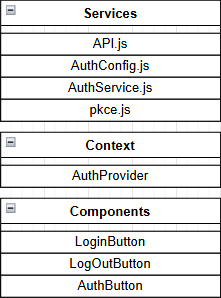
\includegraphics[width=5cm]{./img/fileStructure.png}
\end{center}


Der Login-Prozess wird in drei semantische Kategorien aufgeteilt. An erster Stelle stehen die Komponenten,
die dem Nutzer die Interaktion mit der Authorisierungs-Logik ermöglichen. 
\subsubsection{Components}
Obwohl theoretisch auch eine einzelne Komponente für den Login-Prozess ausreichen würde, wurde der Login/Logout-Button
im Sinne der Übersichtlichkeit gedrittelt. Der Login- sowie Logout-Button sind sind in der Logik bis auf die ausgeführte Methode identisch: \ref{list:loginbutton}

Der Login-Button, welcher aus der Unternehmens-internen React-Bibliothek entnommen wird, ruft bei Interaktion die \texttt{login()}-Methode 
aus dem Authentifizierungs-Kontext auf, welcher im nächsten Abschnitt beschrieben wird.\break
Der gleiche Prozess findet beim Logout-Button statt, nur dass hier die \texttt{logout()}-Methode aufgerufen wird. \ref{list:logoutbutton}

Diese beiden Komponenten werden dann im AuthButton kombiniert, wobei der Auth-Status entscheidet, 
welcher Button angezeigt wird: \ref{list:authbutton}
Für die Entscheidung, welcher Button angezeigt wird, wird zuerst über die \texttt{useAuth()}-Hook\footnote{In JavaScript, speziell in React, ist eine Hook eine Funktion, mit der ein Zugriff auf React-Features wie State oder Lifecycle-Methoden in Funktionskomponenten möglich gemacht wird}
der Authentifizierungs-Kontext abgerufen. Der daraus resultierende Boolean-Wert \texttt{isAuthenticated} gibt an, ob der Nutzer eingeloggt ist oder nicht.
Mit diesem Boolean-Wert wird dann entschieden, ob der Login- oder Logout-Button angezeigt wird. Das geschieht in diesem Fall mithilfe eines ternären Operators,
der den Wert von \texttt{isAuthenticated} überprüft und abhängig vom Wert den entsprechenden Button zurückgibt.\footnote{\url{https://developer.mozilla.org/en-US/docs/Web/JavaScript/Reference/Operators/Conditional_operator}}
\subsubsection{Context}
Der Authentifizierungs-Kontext ist ein zentraler Bestandteil der Authorisierungs-Logik. Er stellt die Methoden \texttt{login()} und \texttt{logout()} 
zur Verfügung, ist aber zusätzlich auch für die Verarbeitung des Callbacks von Cognito zuständig.
Zuerst werden für den Kontext die benötigten Hooks importiert und ein Context-Objekt erstellt: \ref{list:authcontextimports} \ref{list:authcontextvariables}
Daraufhin werden für den Kontext relevante Variablen definiert, die den User, den Authentifizierungsstatus und die Tokens enthalten:
Die \texttt{login()}-Methode generiert einen zufälligen State und einen PKCE-Verifier, speichert diese im Session Storage und 
leitet den Nutzer zur Authentifizierungs-URL weiter: \ref{list:authcontextlogin}
Die \texttt{logout()}-Methode löscht den Session Storage und leitet den Nutzer zur Logout-URL weiter: \ref{list:authcontextlogout}
Die \texttt{handleCallback()}-Methode wird aufgerufen, wenn der Nutzer nach der Authentifizierung zurück zur Anwendung geleitet wird.
Das wird durch die \texttt{useEffect()}-Hook realisiert, die prüft, ob der Nutzer auf der Callback-Route ist und ob ein Code in der URL vorhanden ist. \ref{list:authcontextcallback}
Die \texttt{handleCallback()}-Methode extrahiert den Code und den State aus der URL, vergleicht den State mit dem im Session Storage gespeicherten Wert und tauscht den Code gegen Tokens aus.
Falls der Austausch erfolgreich ist, werden die Tokens im Zustand gespeichert und der Nutzer wird zur Dashboard-Seite weitergeleitet: \ref{list:authcontextcallback2}
Die \texttt{AuthProvider}-Komponente stellt den Authentifizierungs-Kontext für die gesamte Anwendung bereit: \ref{list:authcontextprovider}
Die \texttt{useAuth()}-Hook ermöglicht den Zugriff auf den Authentifizierungs-Kontext in anderen Komponenten der Anwendung.
\subsubsection{Service}    
Der Service-Ordner enthält unterstützende Funktion für die Authorisierung, wie die Generierung des PKCE-Verifiers 
und -Challenges, den Austausch des Codes gegen Tokens und die Erstellung der Authentifizierungs-URL.
Zuerst muss dafür die Konfiguration definiert werden, mit der gearbeitet wird.
\subsubsection{AuthConfig}
Die \texttt{authConfig.js}-Datei enthält die Konfiguration für die Authentifizierung, einschließlich der Endpunkte, Client-ID und Redirect-URI. 
Zusätzlich wird auch die Basis-URL der API definiert, um später API-Anfragen zu ermöglichen:\ref{list:authconfig}
Mit dieser Konfiguration wird nun gearbeitet, um alle weiteren benötigten Daten zu generieren.
\subsubsection{AuthService}
Der AuthService enthält drei Methoden, die für die Authorisierung benötigt werden:
\begin{itemize}
    \item \texttt{buildAuthUrl()}: Diese Methode generiert die Authentifizierungs-URL, die den Nutzer zur Cognito-Anmeldeseite weiterleitet.
    \item \texttt{exchangeCodeForTokens()}: Diese Methode tauscht den erhaltenen Code gegen Tokens aus, die für die Authentifizierung und Autorisierung verwendet werden.
    \item \texttt{refreshTokens()}: Diese Methode aktualisiert die Tokens, wenn sie abgelaufen sind.
\end{itemize}
Die \texttt{buildAuthUrl()}-Methode erstellt die Authentifizierungs-URL, indem sie die Konfiguration und die PKCE-Challenge verwendet: \ref{list:buildAuth}
Die \texttt{exchangeCodeForTokens()}-Methode tauscht bei Rückruf von der Cognito-Authentifizierung den mitgegebenen Code für ein gültiges
Auth-Token. Dieses kann dann verwendet werden, um API-Abfragen durchzuführen: \ref{list:exchangecodefortoken}
Dafür werden zuerst die nötigen Konfigurations-Daten geladen und die Parameter für die URL-Suche definiert. Mit diesen Daten wird dann 
eine Anfrage an den TokenEndpoint gesendet und die Antwort als das Token zurückgegeben, sollten keine Fehler auftreten.
\subsubsection{PKCE}
PKCE(Proof Key for Code Exchange) ist eine Erweiterung des OAuth 2.0-Protokolls, welches zusätzliche Sicherheit für Clients verspricht,
die nicht in der Lage sind, ihre Client-Geheimnisse sicher zu speichern.
Innerhalb dieser Anwendung wird PKCE verwendet, um den Authentifizierungsprozess sicherer zu gestalten. Dies geschieht über zwei Methoden,
\texttt{generateVerifier()} und \texttt{generateChallenge()}, die jeweils den Verifier und die Challenge generieren. \break

Die \texttt{generateVerifier()}-Methode generiert einen zufälligen Verifier, der als Basis für die Challenge dient. Das geschieht, indem 
ein Array von 32 zufälligen Bytes generiert wird, welches dann in einen hexadezimalen String umgewandelt wird: \ref{list:pkceverifier}
Die \texttt{generateChallenge()}-Methode nimmt den Verifier als Eingabe und generiert die Challenge, indem der Verifier in einen SHA-256-Hash umgewandelt wird.
Das Ergebnis wird dann in einen Base64-URL-kodierten String umgewandelt: \ref{list:pkcechallenge}
\subsubsection{API}
Der API-Service ist die Hook \texttt{useApi()}, welche für die Kommunikation mit der Backend-API zuständig ist. 
Sie Kapselt die Methode \texttt{callAPI()} ab, welche den Zugriff auf die Konfigurierte API ermöglicht: \ref{list:callApi}
Die Daten, die aus der \texttt{callApi()}-Methode zurückgegeben werden, können dann in den Komponenten verwendet werden, um die Daten anzuzeigen oder zu verarbeiten.
\subsection{Dynamische Formularlogik und User Interface}
Das User Interface der Anwendung ist in mehrere Komponenten unterteilt, die jeweils für verschiedene Teile der Anwendung zuständig sind:\break
\begin{center}
    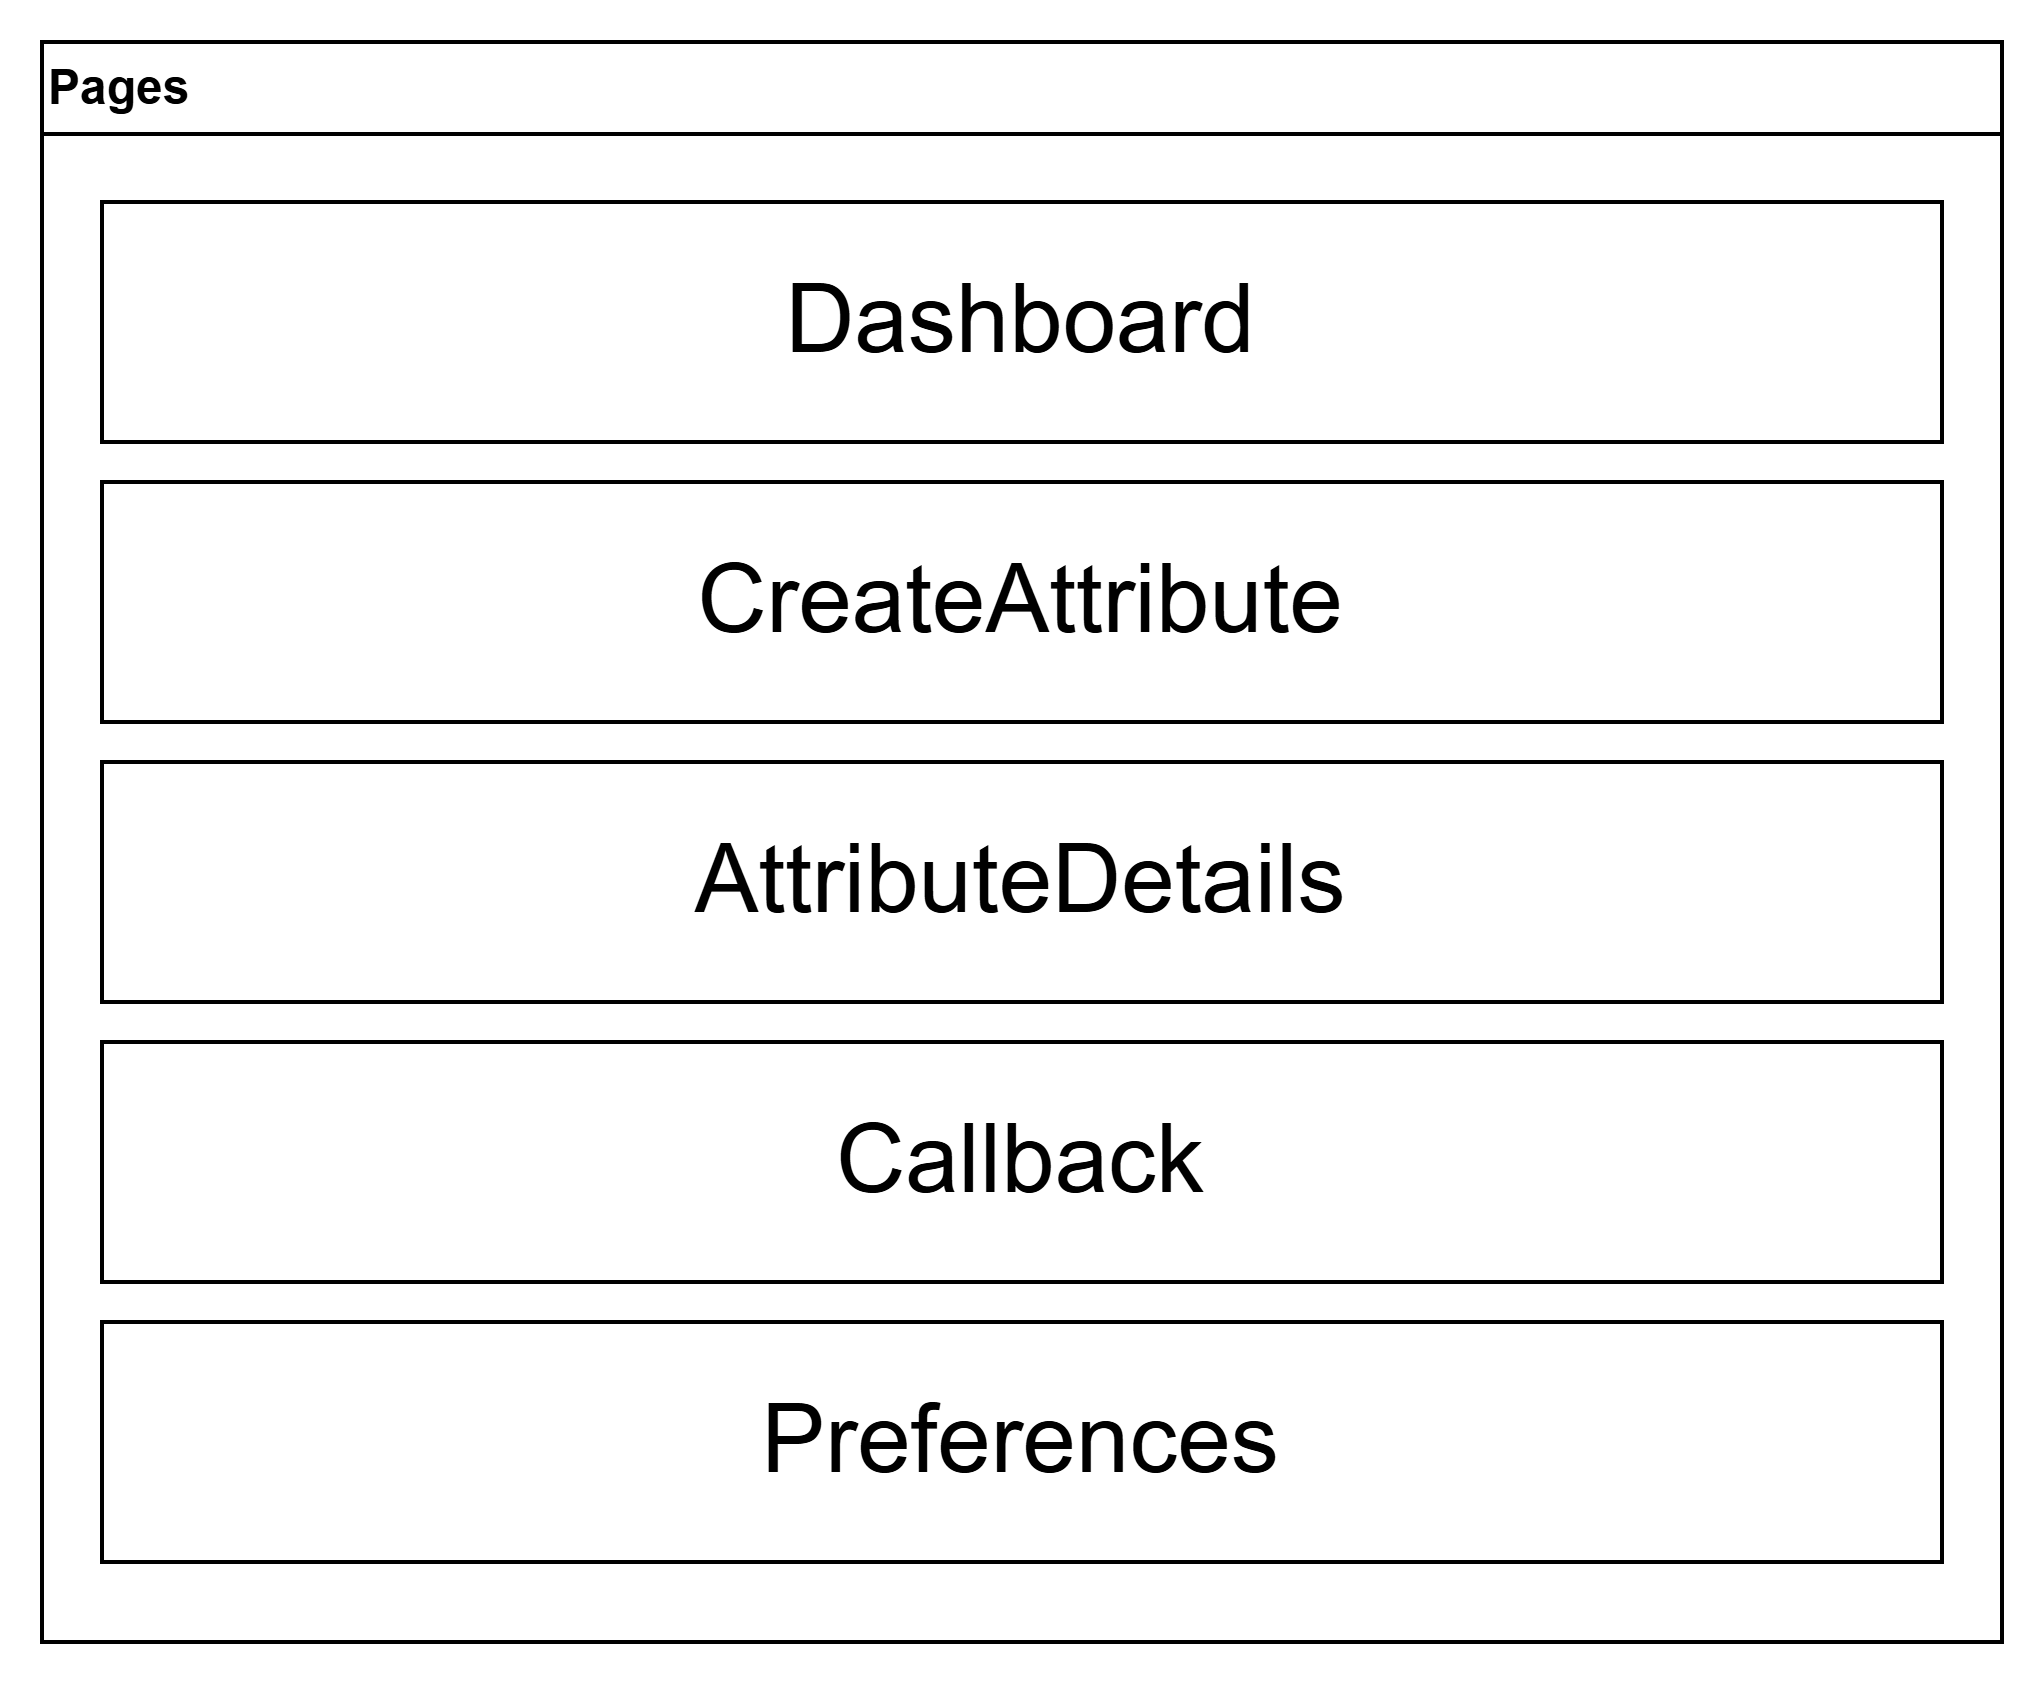
\includegraphics[width=5cm]{./img/dashboardFileStructure.png}
\end{center}
Den Kern der Anwendung bildet die \texttt{Dashboard}-Komponente, welche die Hauptansicht der Anwendung beinhaltet. Von hier aus werden die verscheidenen
Unterseiten aufgerufen (mit Ausnahme der Callback-Seite, die nur für die Authorisierung zuständig ist).
\subsection{Anwendungsbeispiel}
Im Folgenden soll anhand eines konkreten Anwendungsbeispiels die Funktionsweise der Anwendung verdeutlicht werden. Dabei soll gezeigt werden, wie ein Attribut erstellt,
zugeordnet, bearbeitet und gelöscht werden kann. Dadurch soll die Funktionsweise des Systems aus Sicht eines Endnutzers erklärt werden.

\subsubsection{Anlegen eines neuen Attributs}
Um ein neues Attribut anzulegen, navigiert der Nutzer zur \texttt{Attributserstellung}, indem er den entsprechenden Button im Dashboard klickt. 
Daraufhin wird der Nutzer aufgefordert, die erforderlichen Informationen für das Attribut einzugeben. Dabei wird im Hintergrund durch die Anwendung 
die Konformität der Eingaben überprüft, und gegebenenfalls eine Fehlermeldung angezeigt. Durch klicken des \texttt{Next}-Buttons kann der Nutzer dann
die Eingaben bestätigen und die zweite Seite der Attributserstellung aufrufen.
\begin{center}
    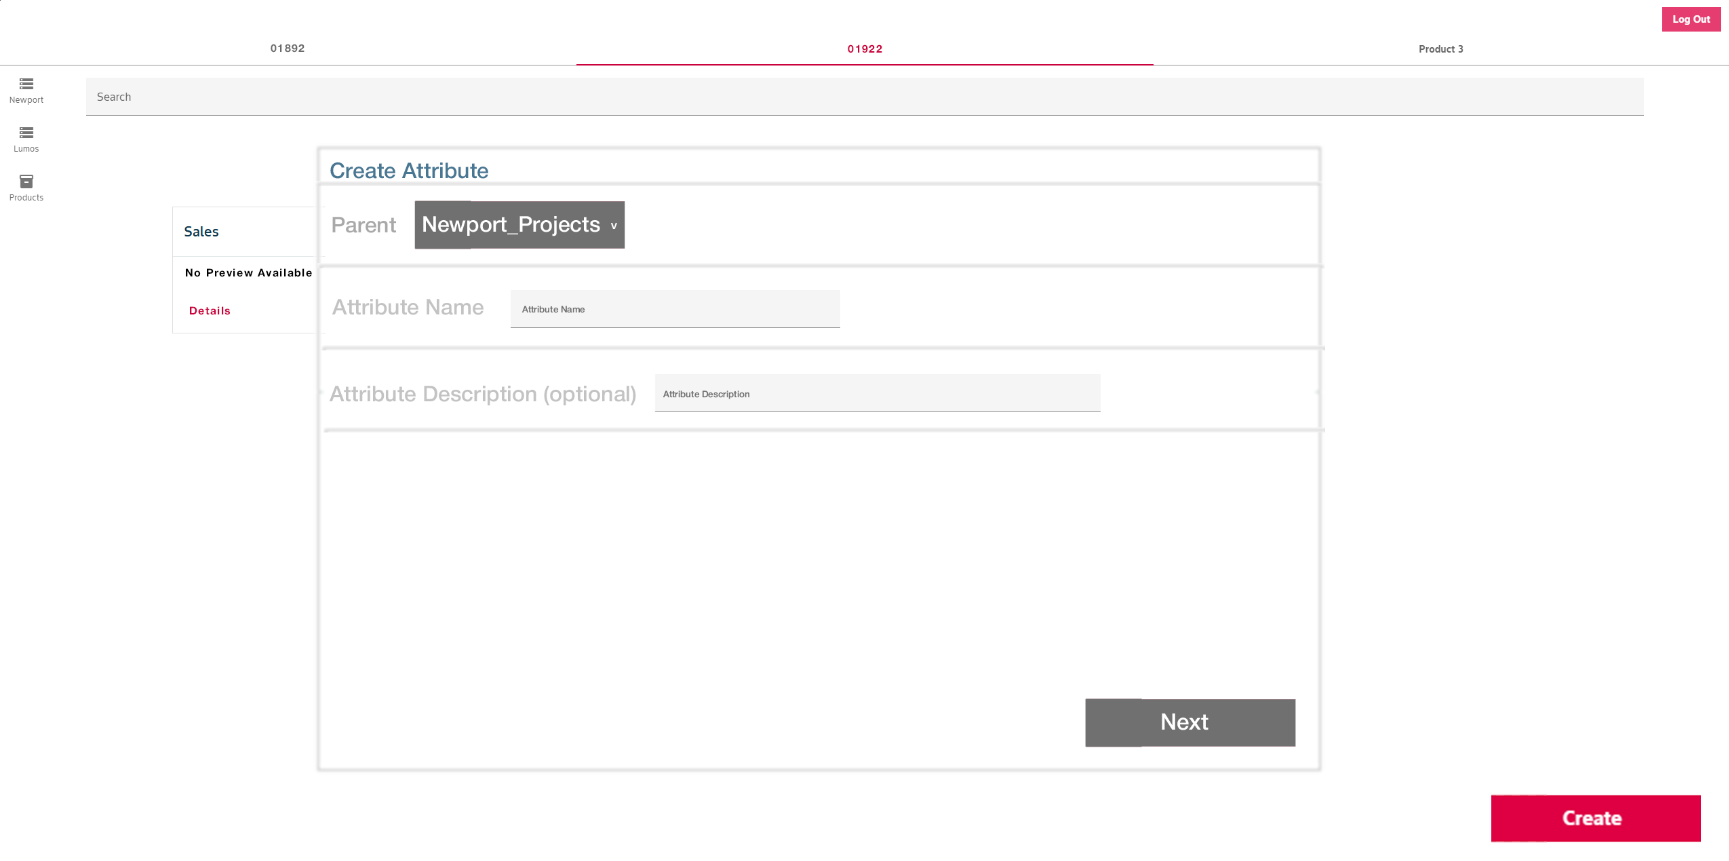
\includegraphics[width=\linewidth]{./img/attributKreation1.png}
\end{center}

Die zweite Seite der Attributserstellung ermöglicht es dem Nutzer, dem Attribut sofort Werte hinzuzufügen. Dafür werden zuerst Informationen über die Art der Werte 
abgefragt, woraufhin der Nutzer die Werte in einer Tabelle eingeben kann. Durch klicken des \texttt{Create}-Buttons kann der Nutzer dann seine Eingaben bestätigen,
und das Attribut wird erstellt. Im Hintergrund wird dafür die API aufgerufen, die das Attribut in der Datenbank anlegt. 

\subsubsection{Bearbeiten eines Werts}
Um einen Wert zu bearbeiten, navigiert der Nutzer zuerst auf die Detailansicht des Attributs, in welchem der Wert enthalten ist. Dort findet er eine Tabelle vor, 
die alle Werte aufführt, und ihm ermöglicht, die Werte zu bearbeiten. Durch klicken des \texttt{Save}-Buttons kann der Nutzer dann seine Änderungen speichern. Im 
Hintergrund wird dafür die API aufgerufen, die den Eintrag in der Datenbank aktualisiert. 
\subsubsection{Löschen eines Attributs}
Um ein Attribut zu löschen, navigiert der Nutzer auf die Detailansicht des Attributs, welches er löschen möchte. Dort findet er einen \texttt{Delete}-Button,
der ihn auffordert, das Löschen zu bestätigen. Nach der Bestätigung wird das Attribut gelöscht, und der Nutzer wird auf die Startseite zurückgeleitet. Im Hintergrund
wird dafür die API aufgerufen, die den Eintrag und alle zugehörigen Referenzen in der Datenbank löscht.
\subsubsection{Zusammenfassung der Attributverwaltung}
Das User Interface ist darauf ausgelegt, dem Nutzer eine einfache und intuitive Möglichkeit zu bieten, Attribute zu erstellen, zu bearbeiten und zu löschen. 
Dafür soll der Nutzer in möglichst wenigen Schritten zu seinem Ziel gelangen, und die Anwendung soll ihn aktiv unterstützen, indem sie im Hintergrund möglichst 
viele Aufgaben übernimmt. Beispielsweise wird die Zugehörigkeit zu einem semantischen Projekt automatisch erkannt, und der Nutzer muss dieses nicht manuell angeben.
\subsection{Herausforderungen und Entscheidungen}

Während der Umsetzung des Frontends sind verschiedene Herausforderungen aufgetreten, die sich nicht nur auf den Code selbst, sondern auch auf Nutzerführung, Fehlerverhalten und Wartbarkeit ausgewirkt haben. Im Folgenden sollen die wichtigsten dieser Punkte - und die Entscheidungen, die daraus resultierten - kurz beschrieben werden.

\subsubsection*{Dynamisches UI ohne Sonderfälle}
Eine der zentralen Fragen war: Wie lässt sich ein Interface bauen, das automatisch auf neue Attribute reagiert, ohne dass man bei jeder kleinen Änderung im Code 
nachbessern muss? Die Lösung bestand darin, Eingabeformulare komplett dynamisch zu generieren - also zur Laufzeit auf Basis der hinterlegten Attribut-Definitionen.  
Das macht den Code insgesamt generischer, aber auch schwerer lesbar. Trotzdem war es die bessere Entscheidung, da so alle Objekte (Formulierungen, Segmente etc.)
 einheitlich behandelt werden können. Anpassungen am Layout einzelner Felder wurden bewusst vermieden, um die Wartbarkeit nicht zu gefährden.

\subsubsection*{Validierung: sofort oder später?}
Ursprünglich war angedacht, die Validierung ausschließlich über das Backend laufen zu lassen - also Fehler erst nach einem Request zurückzumelden. Das führte aber zu 
Frust, weil Nutzer:innen gar nicht wussten, ob ihre Eingaben korrekt sind.  
Deshalb wurde zusätzlich eine einfache Validierung im Frontend umgesetzt: Pflichtfelder, Datentypen und leere Eingaben werden direkt geprüft, bevor überhaupt ein 
Request abgeschickt wird. Dadurch werden Fehler früher abgefangen, ohne dass die API komplett entlastet werden muss.

\subsubsection*{Generik trifft auf Lesbarkeit}
Weil viele Teile des Frontends dynamisch funktionieren müssen, ist der Code an manchen Stellen weniger intuitiv. Zum Beispiel müssen nicht nur Felder, sondern auch 
zugehörige State-Objekte, Event-Handler und API-Requests zur Laufzeit angepasst werden.  
Um das im Griff zu behalten, wurden klare Zuordnungen zwischen Attributtyp und UI-Komponente eingeführt - z. B. dass „Zahl“ immer ein bestimmtes Input-Feld erzeugt. 
Solche Regeln wurden in Hilfsfunktionen ausgelagert, damit die Hauptkomponenten übersichtlich bleiben.

\subsubsection*{Fehlertoleranz bei API-Problemen}
Da das Frontend stark auf die API angewiesen ist, war schnell klar: Wenn eine Anfrage scheitert oder langsam ist, muss das UI trotzdem stabil bleiben.  
Deshalb wurden für alle Requests Lade- und Fehlerzustände eingebaut, die direkt im UI angezeigt werden. Das heißt: Buttons deaktivieren sich automatisch bei 
laufender Anfrage, Fehler werden in Klartext angezeigt - und das System bleibt insgesamt bedienbar, auch wenn das Backend mal nicht reagiert.

\subsection{Fazit zur Frontend-Implementierung}
Im Rahmen des Frontends wurde eine benutzerfreundliche und sichere Anwendung entwickelt, die es Nutzern ermöglicht, Attribute zu erstellen, zu bearbeiten und zu löschen.
Um die Erweiterbarkeit und Wartbarkeit der Anwendung zu gewährleisten, wurde eine modulare Struktur gewählt, durch welche neue Funktionen und Komponenten einfach hinzugefügt
werden können. Die Anwendung ist so konzipiert, dass Nutzer einfach und intuitiv mit ihr interagieren können, während im Hintergrund komplexe Logik und Sicherheitsmaßnahmen
abgearbeitet werden. Dafür wurden folgende Features implementiert:
\begin{itemize}
    \item Dynamische Attributerstellung
    \item Zuweisung von Attributen zu Datenobjekten
    \item Werteingabe und Validierung
    \item Bearbeiten und Löschen von Werten
    \item Dynamisches Rendering von Formularen
    \item API-Kommunikation mit Lade- und Fehlerstatus
    \item Zustandsverwaltung mit React Hooks
    \item Grundlegende Benutzerführung
    \item Selbsterklärende Struktur und Modularität
\end{itemize}
